\documentclass[journal]{IEEEtran}

\ifCLASSINFOpdf
\usepackage[pdftex]{graphicx}
  % declare the path(s) where your graphic files are
\graphicspath{{../pdf/}{../jpeg/}{../eps/}}
  % and their extensions so you won't have to specify these with
  % every instance of \includegraphics
\DeclareGraphicsExtensions{.pdf,.jpeg,.png,.eps}
\else
  % or other class option (dvipsone, dvipdf, if not using dvips). graphicx
  % will default to the driver specified in the system graphics.cfg if no
  % driver is specified.
  % \usepackage[dvips]{graphicx}
  % declare the path(s) where your graphic files areb
  % \graphicspath{{../eps/}}
  % and their extensions so you won't have to specify these with
  % every instance of \includegraphics
  % \DeclareGraphicsExtensions{.eps}
\fi

\usepackage[spanish]{babel}  % activa idioma español

\addto\captionsspanish{
  \renewcommand{\tablename}{Tabla}
}

\usepackage{enumitem}

% *** MATH PACKAGES ***
\usepackage{amsmath}
\usepackage{amssymb}
\usepackage{amsthm}
\interdisplaylinepenalty=2500
% *** SPECIALIZED LIST PACKAGES ***
\usepackage{algorithmic}
% *** ALIGNMENT PACKAGES ***
\usepackage{array}
% *** SUBFIGURE PACKAGES ***
\ifCLASSOPTIONcompsoc
  \usepackage[caption=false,font=normalsize,labelfont=sf,textfont=sf]{subfig}
\else
  \usepackage[caption=false,font=footnotesize]{subfig}
\fi
% *** FLOAT PACKAGES ***
%\usepackage{fixltx2e}
%\usepackage{stfloats}
%\usepackage{dblfloatfix}

%\ifCLASSOPTIONcaptionsoff
%  \usepackage[nomarkers]{endfloat}
% \let\MYoriglatexcaption\caption
% \renewcommand{\caption}[2][\relax]{\MYoriglatexcaption[#2]{#2}}
%\fi
%\let\MYorigsubfloat\subfloat
%\renewcommand{\subfloat}[2][\relax]{\MYorigsubfloat[]{#2}}

% *** PDF, URL AND HYPERLINK PACKAGES ***
\usepackage{url}

% correct bad hyphenation here
\hyphenation{op-tical net-works semi-conduc-tor}
\hyphenation{maxi-mizar REINFORCE}

\newtheorem{definition}{Definición}
\newtheorem{theorem}{Teorema}
\newtheorem{lemma}{Lema}
\newtheorem{proposition}{Proposición}

% Corolarios
\newtheorem{corollary}{Corolario}

\begin{document}
%
% paper title
% Titles are generally capitalized except for words such as a, an, and, as,
% at, but, by, for, in, nor, of, on, or, the, to and up, which are usually
% not capitalized unless they are the first or last word of the title.
% Linebreaks \\ can be used within to get better formatting as desired.
% Do not put math or special symbols in the title.
\title{Formalización y Resolución del Problema del Comerciante Holandés}
%
%
% author names and IEEE memberships
% note positions of commas and nonbreaking spaces ( ~ ) LaTeX will not break
% a structure at a ~ so this keeps an author's name from being broken across
% two lines.
% use \thanks{} to gain access to the first footnote area
% a separate \thanks must be used for each paragraph as LaTeX2e's \thanks
% was not built to handle multiple paragraphs
%

\author{Darío Hernández Cubilla,
        Francisco Préstamo Bernardez,
        Jossué Arteche Muñoz
}

% make the title area
\maketitle
% As a general rule, do not put math, special symbols or citations
% in the abstract or keywords.
% \begin{abstract}
% The abstract goes here.
% \end{abstract}

% Note that keywords are not normally used for peerreview papers.
% \begin{IEEEkeywords}
% IEEE, IEEEtran, journal, \LaTeX, paper, template.
% end{IEEEkeywords}

\section{Introducción}
\IEEEPARstart{E}{l} presente trabajo aborda la optimización de la planificación comercial de una expedición marítima, considerando decisiones de ruta y de transacciones en puertos con distintos precios de compra y venta. La investigación se centra en el desarrollo de metodologías para maximizar el capital final de la expedición, bajo restricciones operativas y temporales.

Se propone un enfoque en dos fases: en primer lugar, la búsqueda de rutas factibles y potencialmente rentables; en segundo lugar, la evaluación de la ganancia máxima asociada a cada ruta mediante técnicas de optimización. Para contrastar soluciones exactas con aproximaciones eficientes, se implementa una versión de fuerza bruta y un modelo basado en redes neuronales que aprende a seleccionar rutas con alto potencial de ganancia.

El artículo analiza la correctitud de los métodos propuestos, discute la complejidad algorítmica y compara experimentalmente los resultados obtenidos por los distintos enfoques, proporcionando una visión completa de la viabilidad práctica de las soluciones.

\section{Definición del problema}
A continuación se presenta una descripción informal del desafío abordado en este trabajo, al cual le damos por nombre \textit{Problema del Comerciante Holandés}, siguiendo la narrativa histórica que lo inspira.

\begin{quote}
    La prestigiosa Compañía Holandesa de las Indias Orientales, en su afán por dominar el comercio mundial, se enfrenta a un desafío monumental. Un capitán experimentado, al mando de una de sus valiosas flotas, debe emprender una expedición comercial que partirá de Ámsterdam y, tras recorrer los puertos más lucrativos del Viejo y Nuevo Continente, deberá regresar a su puerto de origen. Los inversores de la Compañía han proporcionado un capital inicial considerable y han establecido un plazo máximo para la duración de la expedición. El capitán tiene la libertad de elegir qué puertos visitar y en qué orden, con la única condición de no visitar el mismo puerto dos veces en el mismo viaje (por cuestiones de acuerdos comerciales y evitar saturación del mercado). En cada puerto, el capitán encontrará una lista de mercancías disponibles, con sus respectivos precios de compra y venta (que pueden variar significativamente). El capitán puede vender las mercancías que lleva a bordo y comprar nuevas. Sin embargo, debe ser astuto:
    \begin{itemize}
        \item La capacidad de carga de su barco es limitada, por lo que no puede llevar más de lo que su bodega permite.
        \item No es necesario vender todas las mercancías al llegar a un puerto; el capitán puede decidir retener parte de su cargamento si cree que podrá venderlo a un precio más alto en un puerto posterior.
        \item Debe asegurarse de que, después de cada operación de compra, le quede suficiente dinero para cubrir los salarios de la tripulación, los impuestos portuarios y las posibles reparaciones del barco hasta el siguiente destino.
        \item El tiempo es oro; la duración total del viaje, incluyendo el tiempo de navegación entre puertos, no debe exceder el plazo fijado por los inversores. El objetivo del capitán es claro: planificar la ruta y las transacciones en cada puerto de tal manera que, al regresar a Ámsterdam, el capital final de la expedición sea el máximo posible, superando con creces la inversión inicial.
    \end{itemize}
\end{quote}
Con base en la descripción informal previa, se presenta una formulación matemática rigurosa del problema y sus soluciones. 

\begin{definition}[Problema del Comerciante Holandés]
    Una instancia del problema del Comerciante Holandés (en adelante CH) se define como una tupla:
    $$
    \mathcal{I} = (V, t, \kappa, S, M, w, p^+, p^-, c^+, c^-, B, v_0, f_0, T)
    $$
    
    donde:
    \begin{itemize}
        \item $V$ es un conjunto de vértices de un grafo completo, que representan los puertos \cite{diestel2005}.
        \item $t : V \times V \to \mathbb{R}^+$ representa el tiempo de viaje entre pares de ciudades.
        \item $\kappa : V \times V \to \mathbb{R}^+$ representa el costo de viaje entre pares de ciudades.
        \item $S : V \to \mathbb{R}^+$ es el costo fijo de visitar cada puerto.
        \item $M$ es el conjunto de mercancías.
        \item $w : M \to \mathbb{R}^+$ es el peso de una unidad de mercancía.
        \item $p^+ : V \times M \to \mathbb{R}^+$ es el precio de compra de una mercancía por puerto.
        \item $p^- : V \times M \to \mathbb{R}^+$ es el precio de venta de una mercancía por puerto.
        \item $c^+ : V \times M \to \mathbb{Z}_{\ge 0}$ es la oferta máxima de una mercancía por puerto.
        \item $c^- : V \times M \to \mathbb{Z}_{\ge 0}$ es la demanda máxima por puerto.
        \item $v_0 \in V$ es el puerto de salida y regreso.
        \item $f_0 \in \mathbb{R}^+$ es el capital inicial.
        \item $B \in \mathbb{R}^+$ es la capacidad del barco.
        \item $T \in \mathbb{R}^+$ es el tiempo límite del viaje.
    \end{itemize}
\end{definition}

\begin{definition}[Solución de CH]
Una solución del problema CH es un par $(R, Q)$
donde:
    \begin{itemize}
        \item $R = (v_{i_0}=v_0, v_{i_1}, \dots, v_{i_r}, v_{i_0})$ es una ruta factible con las condiciones:
            $$
            v_{i_j} \neq v_{i_k} \quad \forall j,k \in \lbrace 1...r \rbrace
            $$ 
            
            $$
            \sum_{j=0}^{r} t(v_{i_j}, v_{i_{j+1}}) \le T
            $$
    (los puertos aparecen a lo sumo una vez en la ruta y el tiempo del viaje no excede el tiempo límite)
        \item $Q$ es un vector de tuplas $Q = ((q^+_1, q^-_1), \dots, (q^+_r, q^-_r))$ de transacciones con funciones
            $$
            q^+_j, q^-_j : M \to \mathbb{Z}_{\geq 0}
            $$
    que representan la compra y venta respectivamente del producto $m$ en el puerto $v_{i_j}$
    \end{itemize}
\end{definition}

También será necesario definir el estado del barco y las restricciones por puerto

\begin{definition}[Estado del barco]
    El estado del barco al llegar al puerto $v_{i_j}$ se define como:
    $$
    \Sigma_j = (f_j, I_j)
    $$
    donde $f_j \in \mathbb{R}_{\ge 0}$ es el capital disponible y $I_j : M \to \mathbb{R}_{\ge 0}$ es el inventario a bordo. El estado inicial es $\Sigma_0 = (f_0, I_0)$ con $I_0(m) = 0$ para toda mercancía $m$.
\end{definition}

\begin{definition}[Restricciones de transición]
    La transición $\Sigma_j \to \Sigma_{j+1}$ se encuentra sujeta a las siguientes restricciones:
\begin{itemize}
    \item Inventario:
        $$
        I_{j+1}(m) = I_j(m) - q^-_j(m) + q^+_j(m) 
        $$
        $$
        I_{j+1}(m) \ge 0
        $$
        $$
        0 \le q^-_j(m) \le I_j(m)
        $$
    \item Capacidad del barco:
        $$
        \sum_{m \in M} I_{j+1}(m)w(m) \le B
        $$
    \item Restricciones de stock del puerto: 
        $$
        0 \le q^+_j(m) \le c^+(v_{i_j}, m)$$
        $$ 
        0 \le q^-_j(m) \le c^-(v_{i_j}, m)
        $$
    \item Capital:
        $$
        f_{j+1} = f_j 
        + C(j)
        - \kappa(v_{i_j}, v_{i_{j+1}}) 
        - S(v_{i_j}) 
        $$
        
        $$
        C(j) = \sum_{m \in M} \lbrack p^-(v_{i_j}, m) q^-_j(m) - p^+(v_{i_j}, m) q^+_j(m) \rbrack 
        $$
        
        $$
        f_{j+1} \ge 0
        $$
\end{itemize}
\end{definition}

Queda definido el problema CH como un problema de optimización con:
\begin{definition}[Función objetivo]
    La función objetivo es maximizar el capital final al retornar al puerto de origen:
        $$
        \max f_{r+1}
        $$    
\end{definition}

Esta formulación integra la planificación de la ruta con las decisiones de compra y venta de mercancías, garantizando que se cumplan todas las restricciones de inventario, capacidad y capital en cada puerto.

\section{Complejidad Computacional}
Para comprender la dificultad intrínseca de CH, se analiza su versión de decisión y se establece su relación con problemas clásicos de optimización combinatoria.

\begin{definition}[CH-DEC]
    Se define el problema de decisión asociado al problema de optimización CH. Dada una instancia
    $$
    \mathcal{I} = (V, t, \kappa, S, M, w, p^+, p^-, c^+, c^-, B, v_0, f_0, T)
    $$
    y un umbral de capital $K \in \mathbb{R}^+$, la pregunta es: ¿existe una solución factible $(R,Q)$ tal que el capital final al regresar al puerto inicial satisfaga
    $$
    f_{r+1} \ge K?
    $$
    Se denotará este problema como CH-DEC.
\end{definition}

Se toma como referencia el conocido \textit{Problema del Viajante} o \textit{Traveling Salesman Problem} (TSP) en su versión de decisión \cite{kleinberg2005}. 

\begin{definition}[Problema del viajante (TSP)]
    Dado un grafo completo $G=(V,E)$ con función de pesos $d:E\to \mathbb{R}^+$ y un umbral $D\in\mathbb{R}^+$, ¿existe un ciclo Hamiltoniano (que visite todos los vértices exactamente una vez) y cuyo costo total no exceda $D$? \cite{diestel2005}.
\end{definition}
El TSP de decisión es un problema conocido NP-completo y por tanto NP-duro \cite{kleinberg2005}

Nótese que el problema requiere visitar un conjunto de puertos sin repeticiones, decidir qué mercancías comprar y vender en cada puerto y planificar la ruta de modo que la secuencia de visitas respete un límite de tiempo total. La combinación de estos elementos sugiere que, para lograr la máxima ganancia, el capitán debe resolver un problema que, en esencia, contiene la dificultad de encontrar un ciclo Hamiltoniano de costo mínimo en un grafo completo ponderado \cite{diestel2005}, es decir, un problema equivalente al TSP. Esta analogía permite entender intuitivamente por qué CH es un problema NP-duro.  

La idea general de la demostración que se presenta a continuación, consiste en forzar a que el comerciante tenga que todos los puertos para recoger todas las unidades de mercancía necesarias para alcanzar $K$. Para esto se crea un grafo donde cada puerto distinto del origen contiene una única unidad de mercancía, el único puerto vendedor es el origen y $K=|V|-1$. Se sigue el esquema para encontrar problemas NP-duros de \cite{kleinberg2005}.

\begin{theorem}
CH es NP-duro.
\end{theorem}

\begin{proof}
Sea una instancia de TSP $(V_{TSP}, d, D)$ con $n = |V_{TSP}|$. Se construye una instancia de CH-DEC como sigue:
    \begin{itemize}
        \item Puertos, tiempos y costos de viaje: $V = V_{TSP}$, $t(u,v) = d(u,v)$, $\kappa(u,v)=0$, puerto inicial $v_0$.
        \item Mercancías: $M=\lbrace m\rbrace$ contiene un único bien con peso $w(m)=1$.
        \item Precios y stock: Para cada puerto $v_i \neq v_0$:
            $$
            c^+(v_i,m) = 1, \quad
            c^-(v_i,m) = 0
            $$
            $$
            p^+(v_i,m) = p^-(v_i,m)= 0
            $$
            
            El puerto $v_0$ se define como el único comprador:
            
            $$
            c^+(v_0,m) = 0, \quad
            c^-(v_0,m) = n-1
            $$
            $$
            p^+(v_0,m) = 0, \quad
            p^-(v_0,m) = 1
            $$
        \item Capacidad, capital e impuestos: $B=+\infty$, $f_0=0$, $S(v)=0$.
        \item Tiempo máximo y umbral de capital: $T=D$, $K=n-1$.
    \end{itemize}

Se demuestra a continuación la equivalencia entre ambas instancias, para demostrar la correctitud de la reducción.

\begin{itemize}
    \item Desde TSP a CH: Sea
        $$
        C = (v_0, v_{i_1}, \dots, v_{i_{n-1}}, v_0)
        $$
    un ciclo Hamiltoniano de costo total $\leq D$.
    Definimos la solución del Comerciante Holandés:
    \begin{itemize}
        \item Ruta: $R = C$.
        \item Transacciones:
          $$
          q^+_j(m) = 1 \quad q^-_j(m) = 0 \quad \text{en cada } v_{i_j}
          $$
          $$
          q^+_j(m) = 0 \quad q^-_{r+1}(m) = n-1 \quad \text{en } v_0
          $$
    \end{itemize}
    Notemos que el inventario se incrementa en una unidad por puerto visitado y nunca es negativo. En el puerto $v_0$, el inventario acumulado es exactamente $n-1$, por lo que la restricción $0 \leq q^-_{r+1}(m) \leq I_{r+1}(m)$ se satisface. Cada puerto $v_i \neq v_0$ permite a lo sumo una compra, por lo que se satisfacen las restricciones de stock. La restricción de capacidad se cumple trivialmente pues $B=+\infty$. Además se cumple la restricción de capital pues $f_{r+1} = (n-1) \cdot 1 = n-1 = K$. Por último, el tiempo coincide con el costo del ciclo TSP y es $\le D = T$.
    
    En consecuencia, la solución es factible y satisface $f_{r+1} \ge K$.
    
    \item Desde CH a TSP: Supóngase que existe una solución factible $(R,Q)$ de CH-DEC en $\mathcal{I}'$ tal que $f_{r+1} \ge K = n-1$ Nótese que:
    \begin{itemize}
        \item El capital solo puede aumentar mediante ventas en $v_0$.
        \item Cada unidad vendida incrementa el capital en exactamente 1.
        \item Cada puerto $v_i \neq v_0$ puede aportar a lo sumo una unidad.
        \item El puerto $v_0$ no aporta mercancía.
    \end{itemize}
    Por tanto, para alcanzar $f_{r+1} \ge n-1$, es necesario recolectar exactamente una unidad en cada puerto $v_i \neq v_0$. Esto implica que todos los puertos $v_i \neq v_0$ son visitados una vez, por tanto se tiene la forma $R = (v_0, v_{i_1}, \dots, v_{i_{n-1}}, v_0)$ y como:
$$
\sum_{j=0}^{n-1} t(v_{i_j}, v_{i_{j+1}})
 \le T = D,
$$
la ruta corresponde a un ciclo Hamiltoniano de costo a lo sumo $D$.
\end{itemize}
La reducción se realiza en tiempo polinomial y establece una correspondencia exacta entre todas las soluciones de TSP y soluciones de CH-DEC. Por lo tanto, CH-DEC es NP-duro y el problema de optimización CH es NP-duro. Esta conclusión justifica la necesidad de algoritmos aproximados o heurísticos para instancias de tamaño realista \cite{kleinberg2005}.
\end{proof}

\section{Asunciones generales}
Además de las restricciones explícitas incluidas en la definición formal del problema, el modelo del CH se apoya en un conjunto de asunciones implícitas que delimitan su alcance y simplifican el análisis teórico. Estas asunciones no alteran la naturaleza combinatoria del problema, pero permiten aislar las fuentes principales de complejidad.

\begin{itemize}
    \item Se asume que el tiempo de viaje entre dos puertos es simétrico, es decir,
        $$
        t(u,v) = t(v,u) \quad \forall u,v \in V.
        $$
    Esta asunción modela un espacio simétrico no dirigido y descarta asimetrías debidas a corrientes, vientos u otras condiciones externas.
    \item El costo de viaje no constituye una magnitud independiente, sino que es proporcional al tiempo de desplazamiento:
        $$
        \kappa(u,v) = \alpha \cdot t(u,v), \quad \alpha \geq 0.
        $$
    En consecuencia, minimizar el costo de transporte y minimizar el tiempo de viaje son objetivos compatibles. Esta asunción evita la existencia de trayectos arbitrariamente largos pero baratos (o cortos y prohibitivamente caros) y refleja un único medio de transporte con comportamiento homogéneo. El factor $\alpha$ es constante en todo el grafo y no depende del puerto, del tramo ni del momento del viaje.
    \item Las operaciones comerciales (compra y venta) y los desplazamientos se realizan sin demoras adicionales. No se modelan tiempos de espera, congestión portuaria ni conflictos operativos. El tiempo total del recorrido fluye exclusivamente como consecuencia de los viajes entre puertos. Asimismo, se asume que precios, tiempos de viaje y costos permanecen constantes durante todo el horizonte de planificación. El modelo es, por tanto, estático y no contempla dinámicas temporales.
    \item El modelo no contempla fuentes de aleatoriedad: no se consideran accidentes, retrasos, pérdidas de mercancía, fluctuaciones de precios ni fallas logísticas. Si bien estas extensiones no están prohibidas conceptualmente, se omiten deliberadamente para mantener el problema dentro de un marco puramente determinista y combinatorio.
\end{itemize}

\section{Metodología general de resolución}
El problema CH combina dos fuentes principales de complejidad: la selección de una ruta factible en el grafo de puertos y la planificación óptima de transacciones comerciales a lo largo de dicha ruta.

Desde un punto de vista algorítmico, resulta natural desacoplar ambas dimensiones y abordar el problema como la composición de dos subproblemas claramente diferenciados:

\begin{itemize} 
    \item Búsqueda de rutas: determinar qué secuencias de puertos visitar, respetando las restricciones de unicidad y tiempo total.
    \item Evaluación de una ruta: dado un recorrido fijo, decidir qué comprar y vender en cada puerto para maximizar el capital final.
\end{itemize}

Esta separación no elimina la dificultad global del problema y permite razonar sobre sus componentes de forma estructurada y analizar distintas estrategias de resolución.

Dado un conjunto de puertos $V$ y un puerto inicial $v_0$, el espacio de soluciones puede verse como el conjunto de todas las rutas factibles
$$
R = (v_0, v_{i_1}, \dots, v_{i_r}, v_0)
$$
que satisfacen la restricción de tiempo. Para cada ruta candidata $R$, se define un subproblema de optimización asociado.

\begin{definition}[Problema de evaluación de ruta]
    Dada una ruta $R = (v_0, v_{i_1}, \dots, v_{i_r}, v_0)$ determinar las transacciones $Q$ que maximizan el capital final $f_{r+1}$ sujeto a las restricciones de inventario, capacidad, stock y capital.
\end{definition}

En consecuencia, el problema original puede expresarse conceptualmente como:
$$
\max_{R \in \mathcal{R}} \text{valor}(R),
$$

donde $\mathcal{R}$ es el conjunto de rutas factibles y  $\text{valor}(R) = \max_Q f_{r+1}(R,Q)$ denota el capital máximo alcanzable, respetando las restricciones, al recorrer $R$.

\section{Enfoque de fuerza bruta}
Una estrategia directa consiste en explorar exhaustivamente ambas dimensiones:
\begin{itemize} 
    \item Enumeración de rutas: considerar todas las permutaciones posibles de subconjuntos de puertos, lo que induce un crecimiento exponencial del espacio de búsqueda \cite{cormen2009, kleinberg2005}.
    \item Evaluación completa de transacciones: para cada ruta, considerar todas las combinaciones posibles de compras y ventas en cada puerto, respetando las restricciones del modelo.
\end{itemize}


Este enfoque es conceptualmente simple, pero computacionalmente intratable incluso para instancias relativamente pequeñas. La explosión combinatoria es doble: exponencial tanto en el número de puertos y como en el número de mercancías y cantidades transaccionadas.


\section{Diseño y Análisis de la Solución de Aprendizaje por Refuerzo}

Este enfoque se enmarca dentro de la categoría de \textit{Neural Combinatorial Optimization}, donde se entrena una red neuronal para construir soluciones heurísticas de alta calidad mediante aprendizaje.

\subsection{Formalización como Proceso de Decisión de Markov (MDP)}

Para aplicar aprendizaje por refuerzo (RL), modelamos la construcción de la ruta del comerciante como un problema de toma de decisiones secuencial \cite{russell2020}.

\begin{itemize}
    \item Estado ($S_t$): El estado en el paso $t$ se define por la tupla $(v_t, \mathcal{I}, \mathcal{V}_t)$, donde:
    \begin{itemize}
        \item $v_t$: Es el puerto actual en el que se encuentra el agente.
        \item $\mathcal{I}$: Representa la información estática de la instancia del problema (matrices de tiempos de viaje, precios de compra/venta, capacidades, límites de tiempo, etc.).
        \item $\mathcal{V}_t$: Es el conjunto de puertos ya visitados o inalcanzables debido a las restricciones de tiempo.
    \end{itemize}
    Se excluye deliberadamente el inventario actual del vector de estado. Este diseño desacopla el problema de navegación (decisiones de la red neuronal) del de comercio (decisiones del evaluador logístico). La red aprende a proponer rutas topológicamente prometedoras.

    \item Acción ($A_t$): La acción corresponde a la elección del siguiente puerto $v_{t+1}$ a visitar.
    \begin{itemize}
        \item El espacio de acciones es el conjunto de todos los puertos disponibles $\mathcal{P} = \{0, \dots, N-1\}$.
        \item Se aplica un \textit{enmascaramiento} para asegurar la validez de las acciones: solo se permite viajar a puertos no visitados tal que el tiempo de viaje más el tiempo de retorno al inicio no exceda el límite $T$.
    \end{itemize}

    \item Transición: Dado el estado actual y la elección del puerto siguiente, el sistema transita determinísticamente al nuevo puerto, determinando el consumo de tiempo.

    \item Recompensa ($R$): La recompensa se modela como el beneficio total obtenido por la ruta completa.
     Tratamos con una recompensa episódica al final de la secuencia. La recompensa $R(\tau)$ para una trayectoria completa $\tau = (v_0, v_1, \dots, v_k, v_0)$ se calcula utilizando el evaluador exacto del problema.
\end{itemize}

\subsection{Arquitectura del Modelo Neuronal}

Utilizamos una arquitectura de red neuronal profunda diseñada para procesar la información de la instancia y tomar decisiones de navegación \cite{Goodfellow-et-al-2016}. El modelo parametriza una política estocástica $\pi_\theta(a|s)$.

\subsubsection{Encoder de Instancia (Context Encoder)}

El primer componente es un codificador que transforma las características crudas de la instancia en un vector de contexto denso (\textit{embedding}).

\begin{itemize}
    \item Entrada: Un vector concatenado que contiene matriz de tiempos de viaje, pesos, precios, capacidades, costos y parámetros globales.
    \item Procesamiento: Un Perceptrón Multicapa (MLP) con funciones de activación ReLU \cite{Goodfellow-et-al-2016}.
    \item Salida: Un vector de características latentes $h_{context}$ que resume la ``topología comercial" del problema.
\end{itemize}

\subsubsection{Policy Network (Actor)}

La red de política decide el siguiente movimiento basándose en el contexto global y la ubicación actual.

\begin{itemize}
    \item Embedding de Puerto Actual: El puerto actual $v_t$ se codifica mediante One-Hot Encoding y se pasa por una capa lineal para obtener un vector denso $h_{port}$.
    \item Decodificador:
    \begin{itemize}
        \item Concatena el contexto de la instancia $h_{context}$ con el embedding del puerto actual $h_{port}$.
        \item Pasa esta información combinada a través de capas densas (MLP).
        \item Salida: Un vector de \textit{logits} de tamaño $N$, que representa la preferencia no normalizada por cada posible puerto destino.
    \end{itemize}
\end{itemize}

\subsubsection{Mecanismo de Enmascaramiento y Selección}

\begin{enumerate}
    \item Se calcula una máscara de validez $M_t \in \{0, 1\}^N$.
    \item Los logits correspondientes a puertos inválidos se establecen en $-\infty$.
    \item Se aplica una función Softmax para obtener una distribución de probabilidad válida:
\end{enumerate}
    \[ \pi_\theta(v_{t+1} | v_t, \mathcal{I}) = \text{Softmax}(\text{Logits}) \]

\subsubsection{Especificaciones Técnicas (V1)}

La implementación inicial en PyTorch \cite{paszke2019pytorchimperativestylehighperformance} se estructura con:
\begin{itemize}
    \item Hiperparámetros Base: Embedding Dim: 128, Hidden Dim: 1024, Optimizador Adam ($10^{-4}$).
    \item Encoder: Linear $\to$ ReLU $\to$ Linear.
    \item Decoder: Linear $\to$ ReLU $\to$ Linear.
\end{itemize}

\subsection{Algoritmo de Entrenamiento Base: REINFORCE}

El entrenamiento base utiliza el algoritmo de gradiente de política REINFORCE \cite{russell2020}, optimizando la esperanza del beneficio $J(\theta) = \mathbb{E}_{\tau \sim \pi_\theta} [R(\tau)]$.

El gradiente se estima mediante:
\[ \nabla_\theta J(\theta) \approx \frac{1}{M} \sum_{i=1}^M \sum_{t=0}^{T-1} \nabla_\theta \log \pi_\theta(a_t^{(i)} | s_t^{(i)}) \cdot (R(\tau^{(i)}) - b) \]
donde $b$ es una línea base (baseline) móvil calculada como promedio exponencial.

\subsubsection{Estrategia de Exploración}
Se implementó una estrategia de Temperature Scaling \cite{sutton2018reinforcement} en la función Softmax:
\[ \pi(a_i) = \frac{\exp(z_i / \tau)}{\sum_j \exp(z_j / \tau)} \]
La temperatura $\tau$ decae exponencialmente de 40.0 a 0.1 durante el entrenamiento, pasando de exploración a explotación.

\subsubsection{Entrenamiento ``On-the-Fly" (Active Search)}
El modelo se entrena específicamente para cada instancia (\textit{Active Search}):

\begin{enumerate}
    \item Inicializa los pesos.
    \item Realiza múltiples iteraciones sobre la misma instancia.
    \item Mantiene un registro de la mejor solución encontrada.
\end{enumerate}

\subsection{Mejora del Modelo: Arquitectura V2 con Memory Replay}

Para mejorar la estabilidad y capacidad de convergencia, se desarrolló una versión actualizada (V2).

\subsubsection{Nueva Arquitectura Profunda (V2)}
Se incrementó la capacidad de la red:
\begin{itemize}
    \item Dimensiones Aumentadas: Embedding: $128 \to 512$, Hidden: $1024 \to 2048$.
    \item Profundidad Adicional: Capas adicionales en el codificador de contexto y decodificador para permitir un razonamiento más abstracto.
\end{itemize}

\subsubsection{Memory Replay: Refuerzo de Soluciones Élite}
Se incorpora un buffer de memoria que almacena las $K=4$ mejores rutas encontradas.
Con frecuencia configurable (cada 4 epochs), se ejecuta una fase de replay:
\begin{enumerate}
    \item Para cada ruta élite en memoria, forzar la generación de la ruta.
    \item Calcular probabilidades con temperatura estable (1.0).
    \item Actualizar la política usando la recompensa almacenada.
\end{enumerate}

Este mecanismo estabiliza el aprendizaje y acelera la convergencia al reforzar patrones exitosos.


\section{Evaluadores}

Dada una ruta fija, el problema de determinar las transacciones óptimas se denomina evaluación de ruta. Dada la secuencia de puertos de la ruta $R$, denotamos el índice del paso en la ruta como $j \in \lbrace 0, \dots, r\rbrace$, donde el puerto visitado en el paso $j$ es $u_j = v_{i_j}$. En esta sección se describen las metodologías propuestas para resolver este subproblema.

\subsection{Evaluación mediante Relajación Lineal}

Para garantizar una resolución eficiente, se aplica una relajación de la restricción de integridad de las mercancías. Se asume que los bienes son infinitamente divisibles (variables continuas en lugar de enteras), lo que permite formular este desafío como un problema de Programación Lineal (LP), el cual tiene conocidos algoritmos con tiempo de ejecución polinomial \cite{cormen2009}. Si bien esta asunción simplifica la realidad física de ciertas mercancías, permite utilizar algoritmos de resolución exactos como Simplex, que en promedio presenta una ejecución eficiente \cite{cormen2009}. 

Se asume asimismo que la ruta $R$ proporcionada como entrada ya satisface las restricciones temporales del problema original.

\begin{theorem}[Formulación del Modelo LP]
\label{thm:lp-model}
El problema de evaluación de caminos donde los bienes son infinitamente divisibles se puede formular como un problema de Programación Lineal
\end{theorem}

\begin{proof}
    Se construye el siguiente modelo de LP para el problema de evaluación de ruta:
    \paragraph*{Variables de decisión}
    Para cada paso $j$ y mercancía $m \in M$:
    \begin{itemize}
        \item $q_{j,m}^+ \in \mathbb{R}_{\ge 0}$: Cantidad comprada de la mercancía $m$ en el paso $j$.
        \item $q_{j,m}^- \in \mathbb{R}_{\ge 0}$: Cantidad vendida de la mercancía $m$ en el paso $j$.
    \end{itemize}
    
    \paragraph*{Variables de estado}
    \begin{itemize}
        \item $I_{j,m} \in \mathbb{R}_{\ge 0}$: Inventario de la mercancía $m$ al salir del puerto en el paso $j$.
        \item $f_j \in \mathbb{R}_{\ge 0}$: Capital disponible después de las transacciones y gastos en el paso $j$.
    \end{itemize}
    
    \paragraph*{Función Objetivo}
    Maximizar el capital acumulado al finalizar la ruta:
    $$
    \text{Maximizar } \quad f_{r+1}
    $$
    
    \paragraph*{Restricciones}
    El modelo está sujeto a las siguientes restricciones para todo $j \in \lbrace 1, \dots, r\rbrace $ y $m \in M$:

    1) \textit{Balance de inventario:} El inventario actual es el anterior más las compras menos las ventas.
    \begin{equation*}
        I_{j,m} = I_{j-1,m} + q_{j,m}^+ - q_{j,m}^-
    \end{equation*}
    
    2) \textit{Capacidad del barco:} El peso total del inventario no puede exceder la capacidad $B$.
    \begin{equation*}
        \sum_{m \in M} I_{j,m} \cdot w(m) \le B
    \end{equation*}
    
    3) \textit{Balance de capital:} El capital se actualiza restando costos de viaje, tasas portuarias y compras y sumando ventas. Se debe garantizar solvencia en todo momento ($f_j \ge 0$).
    \begin{equation*}
    \begin{split}
        f_j = f_{j-1} & - \kappa(u_{j-1}, u_j) - S(u_j) \\
                      & + \sum_{m \in M} \left( p^-(u_j, m) q_{j,m}^- - p^+(u_j, m) q_{j,m}^+ \right) \ge 0
    \end{split}
    \end{equation*}
    
    4) \textit{Límites de mercado:} Las transacciones no pueden exceder la oferta y demanda local del puerto actual.
    \begin{equation*}
        0 \le q_{j,m}^+ \le c^+(u_j, m)
    \end{equation*}
    \begin{equation*}
        0 \le q_{j,m}^- \le c^-(u_j, m)
    \end{equation*}
    
    5) \textit{Consistencia de venta:} No se puede vender más mercancía de la que se transportaba al llegar al puerto.
    \begin{equation*}
        q_{j,m}^- \le I_{j-1,m}
    \end{equation*}
\end{proof}

Con condiciones iniciales $f_0$ dado por la instancia e $I_{0,m} = 0$. Este modelo lineal permite evaluar rápidamente la rentabilidad potencial de una ruta candidata generada por los algoritmos de búsqueda.

Sin asumir la infinita divisibilidad de los bienes, se tendría un problema de programación lineal entero, con el cual se puede evaluar un camino para obtener una solución óptima sin asumir ninguna relajación relajación del problema, sin embargo, este tipo de problemas es NP-duro \cite{cormen2009}.


\subsection{Evaluador con Capital Infinito y sin límites de Compra o Venta}

Se puede asumir que el Comerciante dispone de capital infinito (i.e. puede entrar en deudas) y no tiene límites en la cantidad de productos que puede comprar o vender en cada puerto. Dado esto, es necesario limitar la cantidad de transacciones que puede efectuar en un mismo puerto, pues si no, en un puerto donde exista un precio de venta mayor que el de compra, el Comerciante podría comprar y vender infinitamente dicho producto para obtener ganancias infinitas. Como compromiso, se asume que el Comerciante puede vender lo que ya tiene en el cargamento en un puerto y comprar productos potencialmente iguales en este, pero no viceversa.

Como idea de alto nivel para la demostración de la correctitud del algoritmo de este evaluador, se dividirá el espacio de carga en ``unidades de carga'' indivisibles e independientes, esto es, una unidad de carga puede en cada momento contener una cantidad de peso igual de un único producto (i.e. estar completamente llena), o estar completamente vacía. Se demostrará que se puede descomponer de esa forma cualquier solución y usando el hecho de que para una unidad de carga existe una solución óptima, igualar cualquier solución óptima a una en la que el espacio de carga completo se comporta como una unidad de carga.

\begin{theorem}
    Bajo estas restricciones, existe una solución óptima donde la bodega de carga siempre está completamente llena de un único producto, o completamente vacía.
\end{theorem}

\begin{proof} 
    Primeramente, tómese una instancia del problema, con la restricción de que el cargamento solo puede estar completamente lleno de un mismo producto, o completamente vacío, existe una serie de decisiones que se pueden tomar $S$, que maximizan la ganancia dado un camino, con las restricciones restantes del problema.

    Ahora, tómese una solución óptima del problema sin esta restricción. En una solución óptima, se puede interpretar la bodega de carga como un segmento inicialmente sin color $H$. Cuando se compra un peso $L$ del producto $m_i$, un conjunto de secciones (subsegmentos) sin color de $H$, cuya suma de longitudes es $L$, se colorea con el color $c_i$; y cuando se vende un peso $L$ de un producto $m_i$, tómese de $H$ un conjunto de subsegmentos coloreados con $c_i$, tal que la suma de sus longitudes es $L$ (lo cual debe existir) y se les quita el color. Ahora, se divide $H$ en segmentos que en cada momento fueron o bien completamente de algún color $c_i$ o bien sin color. Dado que la cantidad que se puede comprar o vender en un puerto es infinita, estos segmentos son independientes, esto es, la decisión de llenar o vaciar uno en un puerto dado no afecta la factibilidad de tomar decisiones sobre otros y ninguno de ellos podría haberse utilizado para obtener una ganancia mayor que $S$ por unidad de peso en la bodega, porque entonces $S$ no sería óptima. Por lo tanto, es posible simplemente sustituir las decisiones tomadas sobre cada uno de estos segmentos de carga por las tomadas para toda la bodega en $S$.
    
    Por lo tanto, existe una solución óptima tal que la bodega siempre está llena con un único producto, o completamente vacía.
\end{proof}

\begin{theorem}
    El problema se reduce a un problema de planificación de intervalos ponderados \cite{kleinberg2005}
\end{theorem}

\begin{proof}
    El problema se reduce a lo siguiente: dados pares de precios de compra y venta $b_{im}$, $s_{jm}$ para ciudades $u_i, u_j$ y productos $m$, tales que $i < j$, obtener el conjunto de intervalos no superpuestos $[i, j]$, cada uno con valor $v = s_{jm} - b_{im}$, tal que la suma de sus valores sea máxima, esto es equivalente a buscar decisiones de compras que llenen la bodega o vacíen la bodega, tal que no tengan conflictos y maximicen la ganancia. Este es un problema de planificación de intervalos ponderados (weighted interval scheduling). 
\end{proof}

Se pueden encontrar los intervalos recorriendo cada par de ciudades diferentes en el trayecto y creando intervalos para cada producto, tomando el precio de compra de la primera ciudad y el precio de venta de la segunda. Es posible omitir los intervalos en los que el precio de venta sea menor que el precio de compra. En cualquier caso, la cantidad de intervalos será $O(n^2 m)$, donde $n$ es la cantidad de ciudades y $m$ la cantidad de productos.

Ahora, para cada intervalo, se tienen dos opciones: tomarlo o no. Tomarlo elimina la posibilidad de tomar intervalos que se solapen con él. Resolveremos este problema utilizando programación dinámica. Sean agrupados los intervalos por tiempo de finalización, si se almacena el peso máximo que podemos obtener en el subconjunto de todos los intervalos que terminan en o antes de $i$, para cada $i$, la mejor solución para un tiempo de finalización $t = i + 1$ es o bien tomar uno de los intervalos que terminan en $i + 1$ y la mejor solución para el conjunto de intervalos que terminan en o antes del momento en que dicho intervalo comienza, o bien no tomarlo y simplemente reutilizar $S[i]$.

Sea $S[i]$ el peso máximo que es posible alcanzar con todos los intervalos cuyo tiempo de finalización es menor o igual que $i$, entonces
$$
S[i] = \max(\max_c\lbrace w_{ic} + S[h(c)] \rbrace, S[i - 1]),
$$
donde $w_{ic}$ es el peso del $c$-ésimo intervalo con tiempo de finalización $i$ y $h(c)$ es el tiempo de inicio del $c$-ésimo intervalo con tiempo de finalización $i$.

\begin{figure}[!t]
\centering
\begin{algorithmic}[1]
\STATE \textbf{Entrada} Conjunto de intervalos $I = \lbrace (i,j,w)\rbrace$
\STATE \textbf{Salida} Peso máximo alcanzable

\STATE Construir un diccionario $D$ que asocia cada tiempo de finalización $j$
con la lista de pares $(i,w)$ de intervalos que terminan en $j$

\STATE Inicializar $D \leftarrow \emptyset$

\FORALL{$(i,j,w) \in I$}
    \IF{$j \notin D$}
        \STATE $D[j] \leftarrow \emptyset$
    \ENDIF
    \STATE $D[j] \leftarrow D[j] \cup \lbrace(i,w)\rbrace$
\ENDFOR

\STATE Definir la función $S(x)$:
\IF{$x < 0$}
    \STATE \RETURN $0$
\ENDIF

\STATE $take \leftarrow \max \lbrace \, w + S(i) \mid (i,w) \in D[x] \,\rbrace$
\STATE \RETURN $\max(take,\; S(x-1))$

\STATE \textbf{Resultado final:} $S(|I|-1)$
\end{algorithmic}
\caption{Programación dinámica para el problema de planificación de intervalos ponderados}
\label{alg:weighted-interval-dp}
\end{figure}

\begin{theorem}
    La complejidad temporal del algoritmo es $O(n^2 m (\log n + \log m))$, donde $n$ es la cantidad de puertos y $m$ la cantidad de productos.
\end{theorem}

\begin{proof}
    Para el algoritmo de weighted interval scheduling, la configuración inicial de agrupar los intervalos por tiempo de finalización es $O(n\log n)$, mientras que, como se muestra en la Fig.~\ref{alg:weighted-interval-dp}, el cálculo de \texttt{take} en la función $S$ recorre cada intervalo exactamente una vez; la otra llamada a \texttt{max} corresponde a una llamada recursiva dentro de la programación dinámica. Por lo tanto, la complejidad es $O(n \log n)$.

    Aunque el problema de weighted interval scheduling puede resolverse en $O(N \cdot \log(N))$, aquí $N$ es en realidad $O(n^2 m)$, donde $n$ es la cantidad de puertos y $m$ la cantidad de tipos de productos, esto es, como máximo existen $m$ intervalos por cada par de puertos. Por lo tanto, la complejidad total es $O(n^2 m (\log(n) + \log(m)))$.
\end{proof}

Para obtener no solo el peso máximo sino también la solución, siguiendo el
esquema del algoritmo presentado en la Fig.~\ref{alg:weighted-interval-dp},
almacenamos la mejor solución junto con el peso máximo y componemos las
soluciones tomando o no tomando el intervalo correspondiente en cada tiempo de
finalización.

\subsection{Evaluación greedy asumiendo deudas y capacidad infinita}
Otra forma eficiente de evaluar una ruta $R$ dada y obtener una cota superior, surge al asumir que el barco puede tener inventario infinito o suficientemente grande y que la tripulación puede asumir deudas. Esto es asumir que $B=+\infty$ y eliminar la restricción $f_j \geq 0$, teniéndose que $f\in \mathbb{R}$.

Luego, las únicas restricciones relevantes que permanecen son, la no negatividad del inventario y los límites de stock por puerto.

Dado que nuestra función a optimizar puede ser reescrita como:

$$
f_{r+1} = f_0 + \sum_{m\in M}\sum_{j=1}^r \lbrack p^-(u_j,m) q_j^-(m) - p^+(u_j,m) q_j^+(m)  \rbrack
$$

El modelo bajo las asunciones tomadas posee tres propiedades fundamentales:
\begin{itemize}
    \item La función objetivo es aditiva y no existen restricciones cruzadas entre mercancías distintas. Por lo tanto, la ganancia total se obtiene sumando las ganancias óptimas de cada mercancía tratada de manera independiente.
    \item La ruta impone un orden total sobre los puertos. Las compras solo pueden emparejarse con ventas posteriores en la ruta, lo que introduce una dirección temporal estricta.
    \item Para una mercancía fija, cada unidad comprada en un puerto puede verse como un “recurso” que debe emparejarse con una venta posterior. El beneficio de un emparejamiento $(i,j)$, con $i<j$, es $p^-(u_j,m) - p^+(u_i,m)$.
\end{itemize}

Así, el subproblema para una mercancía se reduce a seleccionar emparejamientos rentables entre compras y ventas, respetando las capacidades máximas.

El principio rector del algoritmo greedy es simple: vender primero donde más caro y comprar primero donde más barato, siempre que el orden temporal lo permita \cite{cormen2009, kleinberg2005}.

Para una mercancía fija, el procedimiento conceptual es el siguiente:
\begin{itemize}
    \item Se consideran los puertos con capacidad de venta disponibles, ordenados por precio de venta decreciente.
    \item Para cada puerto de venta $u_j$, se buscan puertos anteriores $u_i$ con capacidad de compra disponible y precio de compra estrictamente menor.
    \item Se emparejan tantas unidades como sea posible entre el mejor comprador disponible y el mejor vendedor disponible, saturando al menos una de las dos capacidades.
    \item El proceso continúa hasta que no exista ningún emparejamiento con ganancia positiva.
\end{itemize}

\begin{figure}[!t]
\centering
\begin{algorithmic}[1]
\STATE \textbf{Entrada} Instancia $\mathcal{I}$, ruta $\mathcal{R}$
\STATE \textbf{Salida} valor óptimo $f$, decisiones $q^+, q^-$
\STATE $f \leftarrow \mathcal{I}.f_0$
\STATE $A \leftarrow \lbrace \, u_k \mid c_k^- > 0 \,\rbrace$ \COMMENT{Puertos donde es posible vender}

\WHILE{$A \neq \emptyset$}
    \STATE $u_j \leftarrow \arg\max \lbrace\, p_k^- \mid v_k \in A \,\rbrace$
    
    \STATE $B \leftarrow \lbrace \,u_i \mid c_i^+ > 0,\; p_i^+ < p_j^-,\; i < j \,\rbrace$
    \COMMENT{Puertos anteriores donde es posible comprar con ganancia}
    
    \IF{$B = \emptyset$}
        \STATE $A \leftarrow A \setminus \lbrace u_j\rbrace$
        \COMMENT{No es rentable vender en $u_j$}
    \ELSE
        \STATE $u_i \leftarrow \arg\min \lbrace \, p_k^+ \mid u_k \in B \,\rbrace$
        
        \STATE $x \leftarrow \min(c_i^+, c_j^-)$
        
        \STATE $q_i^+ \leftarrow x,\quad q_j^- \leftarrow x$
        \COMMENT{Decisión de compra y venta}
        
        \STATE $c_i^+ \leftarrow c_i^+ - x$
        \STATE $c_j^- \leftarrow c_j^- - x$
        \COMMENT{Actualización de inventarios, $A$ y $B$ cambian}
        \STATE $f \leftarrow f + x (p_j^- - p_i^+)$ 
    \ENDIF
\ENDWHILE
\RETURN $f, (q^+, q^-)$
\end{algorithmic}
\caption{Algoritmo greedy para seleccionar pares de puertos con ganancia máxima}
\label{alg:greedy-ports}
\end{figure}

Antes de demostrar que el algoritmo es correcto se enunciaran algunos lemas auxiliares.

\begin{lemma}[Independencia entre mercancías]
\label{lem:greedy-indep}
Calcular
$$
f^*_{r+1} = \max f_{r+1}
$$
es igual a calcular
$$
f^*_{r+1} = f_0 + \sum_{m\in M} \max F_m 
$$

donde 
$$
F_m = \sum_{j=1}^{r}
\bigl(
p^-(u_j,m)q^-_j(m) -
p^+(u_j,m)q^+_j(m)
\bigr)
$$
\end{lemma}
\begin{proof}

Bajo las asunciones $B = +\infty$ y $f_j \in \mathbb{R}$, las restricciones de factibilidad se descomponen por mercancía, es decir, no existe ninguna restricción que involucre simultáneamente decisiones asociadas a mercancías distintas.

Por lo tanto, maximizar la ganancia total es equivalente a maximizar, de manera independiente, la ganancia asociada a cada mercancía.
\end{proof}

Sea una mercancía $m$ fija. Para cada puerto $u_i$ de la ruta se definen:

\begin{itemize}
    \item $c^+_i \ge 0$: capacidad máxima de compra a precio $p^+_i$.
    \item $c^-_i \ge 0$: capacidad máxima de venta a precio $p^-_i$.
\end{itemize}

Al no poder comprarse más unidades de las que se vende, ni ser óptimo comprar una unidad para no venderla, una solución factible queda completamente caracterizada por un conjunto de emparejamientos unitarios
$$
(i,j), \quad i < j,
$$
donde cada emparejamiento representa una unidad comprada en $u_i$ y vendida en $u_j$, respetando las capacidades $c^+_i$ y $c^-_j$.

La ganancia asociada a una pareja $(i,j)$ es $p^-_j - p^+_i$.

\begin{lemma}[Estructura de solución óptima]
\label{lem:greedy-struct}
Sea $\mathcal{O}$ una solución óptima para una mercancía fija.
    \begin{itemize}
        \item No existen emparejamientos no rentables: Toda unidad emparejada $(i,j)$ en $\mathcal{O}$ satisface $p^-_j - p^+_i \ge 0.$
        \item Saturación de emparejamientos rentables: Para todo puerto $u_j$, si en $\mathcal{O}$ se tiene $q^-_j < c^-_j$, entonces no existe ningún puerto $u_i$ con $i<j$ tal que $q^+_i < c^+_i$ y $p^-_j - p^+_i > 0$
    \end{itemize}
\end{lemma}

\begin{proof} La demostración contempla las dos proposiciones:
    \begin{itemize}
        \item Supóngase que una unidad comprada en $v_i$ se vende en $v_j$ con $p^-_j - p^+_i < 0$. Eliminando dicho emparejamiento se obtiene una solución factible con ganancia estrictamente mayor, contradiciendo la optimalidad. El caso $p^-_j - p^+_i = 0$ puede eliminarse sin afectar la ganancia total.
        \item Si existiera un puerto $u_i$ con $i<j$, capacidad disponible de compra y $p^-_j - p^+_i > 0$, entonces agregar una unidad comprada en $u_i$ y vendida en $u_j$ incrementaría estrictamente la ganancia, contradiciendo nuevamente la optimalidad de $\mathcal{O}$.
    \end{itemize}
\end{proof}

\begin{lemma}[Maximalidad del número de emparejamientos]
\label{lem:greedy-max}
    Las soluciones del algoritmo greedy contienen tantos emparejamientos rentables como cualquier solución óptima.
\end{lemma}

\begin{proof}
    Supóngase que el algoritmo greedy termina con una solución $\mathcal{G}$ y que existe otra solución factible $\mathcal{O}$ con más emparejamientos rentables.

    Entonces, en el momento en que el algoritmo greedy se detiene, no existe ningún par $(i,j)$ con capacidad disponible y $p^-_j - p^+_i > 0$.

    Pero entonces $\mathcal{O}$ tampoco puede contener tal emparejamiento, pues violaría el Lema~\ref{lem:greedy-struct}.

Por lo tanto, ninguna solución óptima puede contener más emparejamientos rentables que la solución greedy.
\end{proof}

\begin{theorem}[Correctitud del algoritmo greedy]
\label{thm:greedy-ok}
El algoritmo greedy descrito produce una solución óptima para el Problema de evaluación de ruta fijando una mercancía $m$ asumiendo $B = +\infty$ y $f_j \in \mathbb{R}$.
\end{theorem}

\begin{proof}
    Consideremos una mercancía fija. Demostraremos por inducción sobre el número de emparejamientos que el algoritmo greedy siempre está por delante de cualquier solución óptima \cite{kleinberg2005}.
    
    En el primer emparejamiento, el algoritmo selecciona el mayor $p^-_j$ posible y el menor $p^+_i$ posible con $i<j$, maximizando la ganancia del primer emparejamiento. Ninguna solución óptima puede obtener una ganancia mayor en su primer emparejamiento.
    
    Supongamos que tras $k$ emparejamientos, la ganancia acumulada del algoritmo greedy es al menos la de cualquier solución óptima parcial con $k$ emparejamientos. En el paso $k+1$, el greedy selecciona el emparejamiento con mayor ganancia disponible restante. Luego, tras el emparejamiento $k+1$, el greedy continúa manteniéndose por delante.

    Por el Lema~\ref{lem:greedy-max}, el greedy realiza tantos emparejamientos como cualquier solución óptima. Por tanto, al finalizar, la ganancia total del greedy es al menos la de cualquier solución óptima.
\end{proof}

\begin{corollary}
    Aplicar el algoritmo greedy de manera independiente a cada mercancía produce una solución óptima global para el Problema de evaluación de ruta
\end{corollary}

\begin{proof}
    La demostración es inmediata dados el Lema~\ref{lem:greedy-indep} y el Teorema~\ref{thm:greedy-ok}
\end{proof}

\begin{theorem}
    El algoritmo descrito tiene una complejidad de $O(|M| r^2)$ con $r = |R|-1$ el número de puertos en la ruta (sin contar el retorno a $v_0$).
\end{theorem}

\begin{proof}
    Para cada mercancía $m$, el algoritmo greedy realiza las siguientes operaciones conceptuales:
    Los puertos se ordenan una vez por precio de venta $p^-_j$(orden decreciente) y también se ordenan una vez por precio de compra $p^+_i$ (orden creciente).
    Esto puede realizarse en  $O(r \log r)$
    
    Para cada puerto de venta $u_j$, el algoritmo recorre los puertos de compra anteriores $u_i$ con $i<j$, filtrando aquellos que tienen capacidad disponible y producen ganancia positiva $(p^-_j > p^+_i)$. Cada par $(i,j)$ se considera a lo sumo una vez. Por lo tanto, el número total de operaciones de emparejamiento está acotado por $O(r^2)$. No se itera unidad por unidad, sino que en cada paso se empareja la máxima cantidad posible. Ambas fases dan un costo total de $O(r \log r + r^2) = O(r^2)$

    Aplicando el algoritmo greedy a cada mercancía, se obtiene una complejidad total de $O(|M|r^2)$
\end{proof}


\section{Resultados y Comparaciones}
\label{sec:results}

Para evaluar cuantitativamente la efectividad de la aproximación basada en aprendizaje por refuerzo, se comparó el capital final obtenido por el agente RL con la solución óptima calculada mediante fuerza bruta. Los experimentos se realizaron sobre instancias con entre 5 y 9 puertos, utilizando tres evaluadores de ganancia distintos: relajación lineal (LP), heurística greedy y programación dinámica por intervalos.

La métrica principal de evaluación fue el \emph{ratio de desempeño} definido como $f_{RL}/f_{BF}$, donde $f_{RL}$ denota la ganancia obtenida por el agente y $f_{BF}$ el óptimo global. Adicionalmente, se analizó la frecuencia con la que el agente alcanza exactamente el óptimo y el comportamiento en la cola inferior de la distribución (peor 5\%), con el fin de caracterizar tanto el desempeño promedio como los casos adversos.

Los resultados descriptivos se resumen en la Tabla~\ref{tab:descriptivos}. En todos los evaluadores considerados, el agente RL alcanza en promedio más del 97\% de la ganancia óptima. En particular, el evaluador greedy presenta un ratio medio del 99.39\% y una mediana cercana al óptimo, mientras que en el caso de programación dinámica por intervalos la mediana alcanza el 100\%, lo que indica que en al menos la mitad de las instancias el agente encuentra una solución óptima o equivalente. Asimismo, se observa que el agente alcanza exactamente el óptimo en aproximadamente entre el 43\% y el 48\% de los casos, dependiendo del evaluador.

La validación inferencial incluyó tres contrastes estadísticos complementarios: 
\begin{enumerate}[label=\roman*), nosep]
    \item una prueba $t$ pareada para detectar diferencias medias \cite{ross2014}, 
    \item un test de no-inferioridad con umbral del 95\%\cite{wellek2010}, y 
    \item un test de equivalencia mediante el procedimiento Two One-Sided Tests (TOST) \cite{wellek2010}.
\end{enumerate}

Los resultados inferenciales se presentan en la Tabla~\ref{tab:inferencial}. La prueba de no-inferioridad, con un umbral del 95\%, rechaza de forma contundente la hipótesis de que el agente sea inferior al óptimo más allá de dicho margen en los tres escenarios evaluados. De manera consistente, el test de equivalencia (TOST) confirma que el desempeño del agente se mantiene dentro de un rango estrecho alrededor de su comportamiento medio.

Por otro lado, la prueba t pareada detecta diferencias estadísticamente significativas entre el capital óptimo y el obtenido por el agente RL, lo cual es esperable dado que el agente no está diseñado para replicar exactamente la solución óptima en todos los casos, sino para aproximarla de forma eficiente. En conjunto, estos resultados permiten concluir que el enfoque propuesto es estadísticamente sólido, altamente competitivo frente al óptimo global y considerablemente más escalable para instancias de mayor tamaño.

\begin{table}[t]
\centering
\renewcommand{\arraystretch}{1.2}
\caption{Desempeño del Agente RL: Estadísticos Descriptivos}
\label{tab:descriptivos}
\resizebox{\columnwidth}{!}{
\begin{tabular}{lcccc}
\hline
\textbf{Evaluador} 
& \textbf{Ratio Medio} 
& \textbf{Mediana} 
& \textbf{Óptimo (\%)} 
& \textbf{Peor 5\%} \\
\hline
LP 
& 97.29\% 
& 99.08\% 
& 46.2\% 
& $< 89.85\%$ \\
Greedy 
& 99.39\% 
& 99.99\% 
& 43.0\% 
& $< 96.94\%$ \\
Intervalos 
& 98.62\% 
& 100.00\% 
& 48.0\% 
& $< 93.24\%$ \\
\hline
\end{tabular}
}
\end{table}

\begin{table}[t]
\centering
\renewcommand{\arraystretch}{1.2}
\caption{Validación Estadística del Desempeño del Agente RL}
\label{tab:inferencial}
\resizebox{\columnwidth}{!}{
\begin{tabular}{lccc}
\hline
\textbf{Evaluador} 
& \textbf{No-Inferioridad} 
& \textbf{Equivalencia} 
& \textbf{t pareada} \\
\hline
LP 
& $p < 10^{-6}$ 
& $p < 10^{-6}$ 
& Significativa \\
Greedy 
& $p < 10^{-6}$ 
& $p < 10^{-6}$ 
& Significativa \\
Intervalos 
& $p < 10^{-6}$ 
& $p < 10^{-6}$ 
& Significativa \\
\hline
\end{tabular}
}
\end{table}

Con el fin de evaluar el comportamiento del modelo durante el proceso de entrenamiento, se realizaron múltiples experimentos orientados a analizar la convergencia de los valores estimados a medida que aumenta el número de epochs. Este análisis resulta fundamental para determinar tanto la estabilidad del aprendizaje como la capacidad del modelo para aproximarse a soluciones óptimas de manera progresiva.

\begin{figure*}[t]
    \centering
    \subfloat{\includegraphics[width=0.5\textwidth]{case_1_log.eps}}\hfill
    \subfloat{\includegraphics[width=0.5\textwidth]{case_3_log.eps}}\hfill
    \subfloat{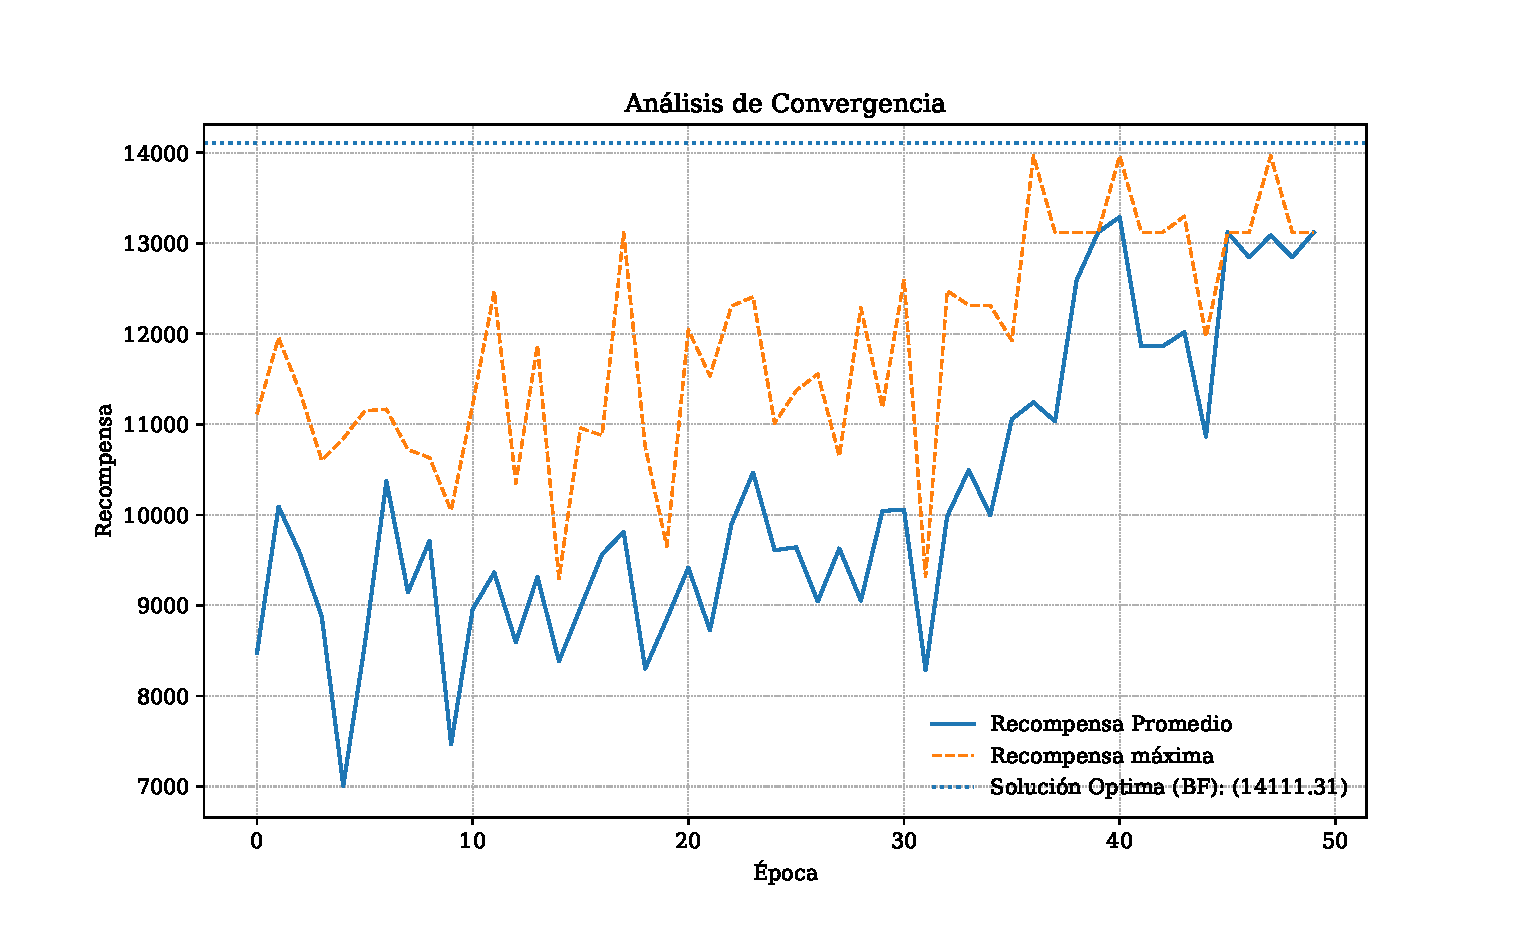
\includegraphics[width=0.5\textwidth]{case_4_log.eps}}\hfill
    \subfloat{\includegraphics[width=0.5\textwidth]{case_5_log.eps}}\hfill
    \subfloat{\includegraphics[width=0.5\textwidth]{case_6_log.eps}}\hfill
    \subfloat{\includegraphics[width=0.5\textwidth]{case_7_log.eps}}\hfill
    \subfloat{\includegraphics[width=0.5\textwidth]{case_8_log.eps}}\hfill
    \subfloat{\includegraphics[width=0.5\textwidth]{case_9_log.eps}}\hfill
    \caption{Convergencia del modelo de aprendizaje por refuerzo en distintos casos de prueba, comparando la evaluación estimada con la solución óptima obtenida por fuerza bruta.}
    \label{fig:convergence}
\end{figure*}

En la figura~\ref{fig:convergence} se muestran algunos casos de prueba representativos en los que se compara la evaluación producida por el modelo de aprendizaje por refuerzo con la solución óptima correspondiente, obtenida mediante un enfoque de fuerza bruta. Esta comparación permite cuantificar de forma directa la calidad de las políticas aprendidas y su evolución a lo largo del entrenamiento.


En todos los escenarios considerados se observa una tendencia consistente de convergencia, donde el valor estimado por el modelo se aproxima gradualmente a un valor cercano al óptimo conforme avanza el proceso de entrenamiento. Este comportamiento sugiere que el modelo es capaz de capturar adecuadamente la estructura del problema y de mejorar su desempeño de manera sostenida a lo largo de las epochs, independientemente del caso de prueba analizado. El modelo mantiene en todo momento el valor máximo encontrado, no solo el valor de la última epoch.


\section{Conclusiones}
En este trabajo se presentó una formulación formal del problema El Comerciante Holandés, integrando decisiones de ruteo y transacciones comerciales en un único marco combinatorio. Se demostró que el problema es NP-duro mediante una reducción directa desde el Traveling Salesman Problem, lo que justifica la necesidad de enfoques aproximados o descomposiciones estructurales.

Con este objetivo, se propuso una metodología basada en separar la búsqueda de rutas de su evaluación económica. Bajo esta perspectiva, se introdujeron distintos evaluadores de caminos que bajo asunciones relajadas, resuelven óptimamente el subproblema de maximización de ganancia para una ruta fija. Esta descomposición permite explorar el espacio de soluciones de manera eficiente y ofrece una base sólida para el diseño de heurísticas prácticas.

\bibliographystyle{ieeetr}
\bibliography{references}

\end{document}